\documentclass[12pt,french]{article} %ajouter draft pour voir débordement
\usepackage[utf8]{inputenc}
\usepackage[T1]{fontenc}
\usepackage{lmodern}
%règles mes marges et format papier
\usepackage[a4paper,hmargin=2cm,vmargin=2cm]{geometry} %modif marge et formet
\usepackage{amsmath, amssymb, amsthm}
\usepackage{fancyhdr} %pour les entêtes et bas de page
\usepackage{lastpage} %pour numéroter les pages charge la derniere page
\usepackage{graphicx} %pour inclure des img
\usepackage{dsfont}
\usepackage{float} %pour le placement des figures
\usepackage{hyperref} %pour mettre des liens hypertext
\usepackage{calc} %permet de calculer les marges pour encadrer les textes
\usepackage{color, xcolor} %gère les couleurs
\usepackage{babel}
\usepackage{listings} %pour afficher le code annexe

%pour afficher le code de manière esthétique
\lstset{
  aboveskip=3mm,
  belowskip=-2mm,
  backgroundcolor=\color{white},
  basicstyle=\footnotesize,
  breakatwhitespace=false,
  breaklines=true,
  captionpos=b,
  commentstyle=\color{red},
  deletekeywords={...},
  escapeinside={\%*}{*)},
  extendedchars=true,
  framexleftmargin=16pt,
  framextopmargin=3pt,
  framexbottommargin=6pt,
  frame=tb,
  keepspaces=true,
  keywordstyle=\color{blue},
  language=C,
  literate=
  {²}{{\textsuperscript{2}}}1 {⁴}{{\textsuperscript{4}}}1
  {⁶}{{\textsuperscript{6}}}1
  {⁸}{{\textsuperscript{8}}}1
  {€}{{\euro{}}}1 {é}{{\'e}}1 {è}{{\`{e}}}1 {ê}{{\^{e}}}1 {ë}{{\¨{e}}}1
  {É}{{\'{E}}}1 {Ê}{{\^{E}}}1 {û}{{\^{u}}}1 {ù}{{\`{u}}}1 {â}{{\^{a}}}1
  {à}{{\`{a}}}1 {á}{{\'{a}}}1 {ã}{{\~{a}}}1 {Á}{{\'{A}}}1 {Â}{{\^{A}}}1
  {Ã}{{\~{A}}}1 {ç}{{\c{c}}}1 {Ç}{{\c{C}}}1 {õ}{{\~{o}}}1 {ó}{{\'{o}}}1 
  {ô}{{\^{o}}}1 {Õ}{{\~{O}}}1 {Ó}{{\'{O}}}1 {Ô}{{\^{O}}}1 {î}{{\^{i}}}1
  {Î}{{\^{I}}}1 {í}{{\'{i}}}1 {Í}{{\~{Í}}}1,
  morekeywords={*,...},
  numbers=left,
  numbersep=10pt,
  numberstyle=\tiny\color{black},
  rulecolor=\color{black},
  showspaces=false,
  showstringspaces=false,
  showtabs=false,
  stepnumber=1,
  stringstyle=\color{gray},
  tabsize=4,
}
%%%%%

%Personalisation En tête
\pagestyle{fancy}
\renewcommand\headrulewidth{1pt}
%permet d'aumenter tailler header pour mettre image (31pt ici)
\setlength{\headheight}{31pt} 
\fancyhead[L]{Architecture Logiciel \\ et Qualité}
\fancyhead[C]{
\includegraphics[scale=0.28]{header.png}}
\fancyhead[R]{Dossier Conception \\ Implémentation}
\renewcommand\footrulewidth{1pt}
\fancyfoot[L]{SMAirport}
\fancyfoot[C]{\thepage/\pageref{LastPage}}
\fancyfoot[R]{2022/2023}
%Fin personalisation En Tête


\begin{document}

\begin{titlepage} %page d'acceuil

  
  
\includegraphics[scale=0.6]{isima.png}
  \hspace*{\stretch{1}}%espace horizontal entre les 2 images
  
\includegraphics[scale=0.2]{deco.jpg}
  
  \vspace*{2.5cm} %espace de 2.5cm en dessous des images
  
  \begin{center}\huge
    \textbf{Dossier Conception Implémentation} 
    
    \textbf{SMAirport}
  \end{center}
  
  \hrule %trait horizontal
  
  \begin{center}
    \Large BALLEJOS Lilian,
    \Large CHARPIN Etienne et
    \Large DENIZOT Hugo
    
    \large
    
    ISIMA INP
  
    Année Universitaire 2022/2023
  \end{center}
  
  \begin{center}
    %créer une boite ou mettre l'image qui fait la largeur de la page
    \makebox[\textwidth]{
\includegraphics[width=\paperwidth]{garde.png}}
  \end{center}
  
  \vspace*{2cm} 
  
  \begin{flushright}\footnotesize %a droite
    Enseignant référant: Mr HILL David
    
    Date du rendu: 17 Avril 2023
    
  \end{flushright}
  
  \begin{flushleft}\small %a gauche
    \textbf{ISIMA}
    \footnotesize
    
    1 rue de la Chebarde - TSA 60125 - CS 60026 - 63178 Aubière CEDEX
    
    Tel: 04 73 40 50 00
    
    Site web: \href{https://www.isima.fr/}{isima.fr}\newline
    	
  \end{flushleft}
\end{titlepage}	


%Ma table des Matières !
%permet de renommer 'table des matières' en sommaire
\renewcommand{\contentsname}{Sommaire}
\normalsize\tableofcontents %place la table des matières

\bigskip

\newpage
\section{Introduction}

Nous allons vous présenter aujourd'hui dans ce dossier la conception programme de \textbf{SMA} (simulation multi-agents).

\bigskip

Il s'agit d'une simulation qui est composée de douaniers et de clients lambdas qui interagiront les uns avec les autres dans un aéroport.

\bigskip

 Nous nous sommes concentrés sur les différents enregistrements que les clients doivent passer, notamment les files d'attente, les fouilles de sécurité et la déposition des bagages. Nous allons également prendre en compte les actions possibles pour les différents agents, comme les douaniers qui peuvent fouiller les clients et les arrêter s'ils ne sont pas en règle. L'objectif de ce projet est d'analyser les différents processus et les interactions entre les agents pour comprendre comment ils contribuent au bon fonctionnement de l'aéroport.
 
 \bigskip
 
 \textbf{Remarque:}
 

Notre projet est disponible sur le Gitlab de l'ISIMA INP en protection \textit{internal} ce qui signifie que pour y accéder il faut être connecté à celui-ci.

Retrouver notre projet en suivant ce lien: \href{https://gitlab.isima.fr/liballejos/smairport}{ici}

\newpage

\section{Choix du langage}

Nous avons décidé de coder ce programme en \textbf{C++} pour deux raisons:

\medskip

\begin{itemize}
	\item Ce langage est performant car plus proche de la machine et sera donc plus efficace et plus rapide pour effectuer une SMA (des programmes qui sont parfois très lourd)
	
	\item Cela nous permettra de nous améliorer dans ce langage que nous étudions en ce moment en cours et sur lequel nous serons évalués.
\end{itemize}


\section{Objectifs}

Nous sommes dans la zone d'entrée d'un aéroport.

L'agent "Client" se déplace entre les différentes parties de l'aéroport et interagit avec celles-ci .

L'agent douanier lui interagit avec les clients en les fouillant et les arrête si ceux-ci ne sont pas en règle.


\section{Implémentation}


\begin{figure}[H]
	\centering
	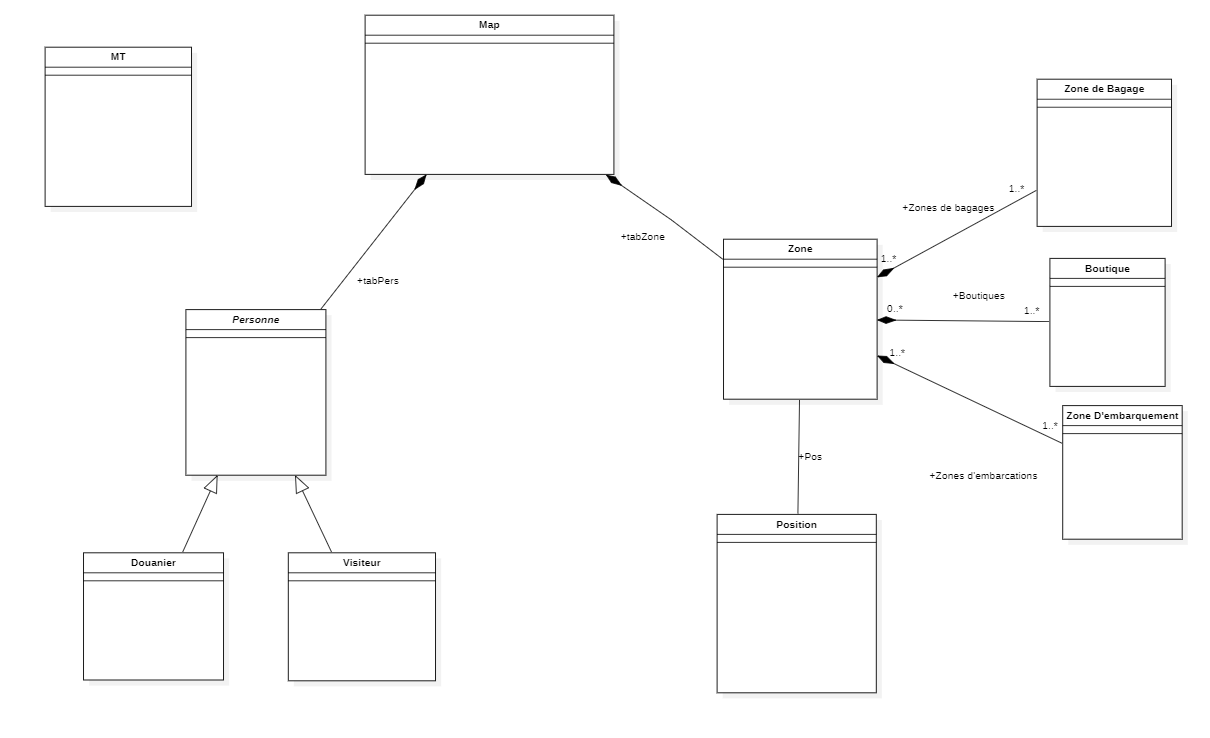
\includegraphics[scale=0.4]{analyse.png}
	\caption{Diagramme de classe de l'application}    
\end{figure}



Pour ce qui est de l'implémentation de notre code, nous avons débuté par le code de nos classes mères. Nous avons dans un premier temps implémenté les classes Zone et Personne pour permettre de les faire hériter sur ZoneBagage, ZoneEmbarquement et Boutique pour l'un et Douanier et Visiteur pour l'autre. Une fois les prototypes de ces classes définis, nous avons choisi de coder la carte de notre aéroport qui se trouve être une grille de 20 cases par 20. Ensuite nous avons pris le temps de coder les déplacements des différentes personnes de notre simulation. Un douanier se déplace alors possiblement à chaque itération d'une case dans tous les sens et cherche si il possède des visiteurs à une case de lui. Si il possède des visiteurs dans son entourage, il en choisit 1 aléatoirement et a une certaine possibilité de le contrôler. Si il est en contrôle, il bloque ses déplacements pendant 2 itérations ainsi que celles du visiteur.
\newline

Concernant l'implémentation de la gestion du tirage aléatoire, nous avons de nouveau utilisé les classes de Mersenne-Twister afin de travailler avec un générateur de nombre pseudo aléatoire efficace.
\newline


Pour le déplacement du visiteur, le principe est sensiblement le même. Comme nous assignons à sa création un temps avant envol, nous avons considéré que le visiteur peut aller visiter une boutique si le temps lui permet, puis devra déposer ses bagages avant d'aller à la zone d'embarquement. Dans sa course, le visiteur peut donc être contrôlé par un douanier ce qui peut potentiellement lui faire rater son avion. C'est cette statistique que nous étudieront dans nos résultats en fin de rapport. Lorsque le visiteur possède un temps suffisant pour aller à une boutique, nous tirons aléatoirement une boutique vers laquelle le visiteur se déplacera.
\newline



Sur l'image ci-dessous, le X représente un visiteur, le D un douanier, le B une boutique, le L un zone de dépot de bagages et enfin le Z pour la zone d'embarquement.


\begin{figure}[H]
	\centering
	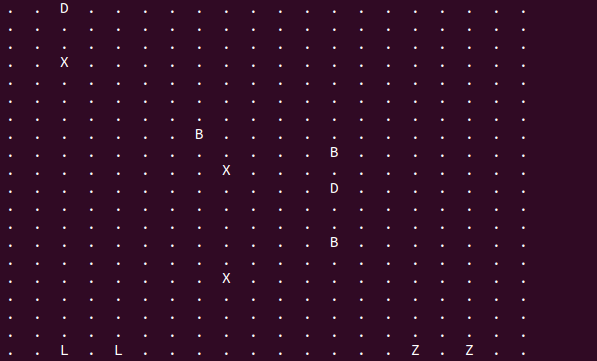
\includegraphics[scale=0.5]{mp.png}
	\caption{Représentation graphique de l'application}    
\end{figure}

\section{Patrons de conception}

Pour ce projet, nous devions choisir et implémenter un ou plusieurs patrons de conception nécessaire à notre développement. Nous avons choisi par nécessité le patron de conception Singleton.

\subsection{Singleton}

\subsubsection{Présentation}

Le Singleton est un patron de conception de création qui garantit que l’instance d’une classe n’existe qu’en un seul exemplaire, tout en fournissant un point d’accès global à cette instance.

\begin{figure}[H]
	\centering
	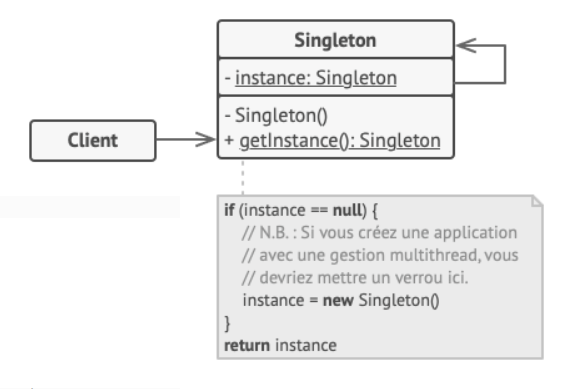
\includegraphics[scale=0.5]{single.png}
	\caption{Diagramme de classe du singleton}    
\end{figure}

\subsubsection{Implémentation}

Dans notre projet, après la mise en place de la conception, nous nous sommes rendu compte de la nécessité d'implémenter un objet Map représentant la carte de l'aéroport. Cette carte se devait d'être disponible pour l'ensemble des agents ainsi qu'aux objets la demandant. En c++, afin de déclarer un objet global, nous devons tout d'abord le déclarer dans la fonction main afin de la créer puis il nous faut ensuite déclarer dans chaque classe nécessitant la Map l'intitulé \textbf{extern Map m}.

\begin{figure}[H]
	\centering
	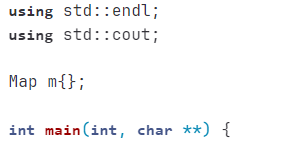
\includegraphics[scale=1]{map.png}
	\caption{Déclaration de notre Map}    
\end{figure}
\section{Résultats}

Afin d'ajouter une utilité à cette simulation multi-agent, nous avons implémenté un petit programme annexe afin de vérifier sur une journée le nombre de personnes ratant leur avion. Nous mettons de coté ceux qui le rate à cause d'un contrôle de douanier. Pour ce faire, nous avons implémenté une journée de 86400 itérations dans un aéroport comportant 2 douaniers 3 boutiques ainsi que 2 zones de bagages et 2 zones d'embarquement. Nous afficherons alors le nombre de personnes ratant leur avion sur le nombre total de personnes venues dans l'aéroport puis nous isolons le nombre de contrôle ainsi que le nombre d'avions ratés à cause d'un contrôle. 



\begin{figure}[H]
	\centering
	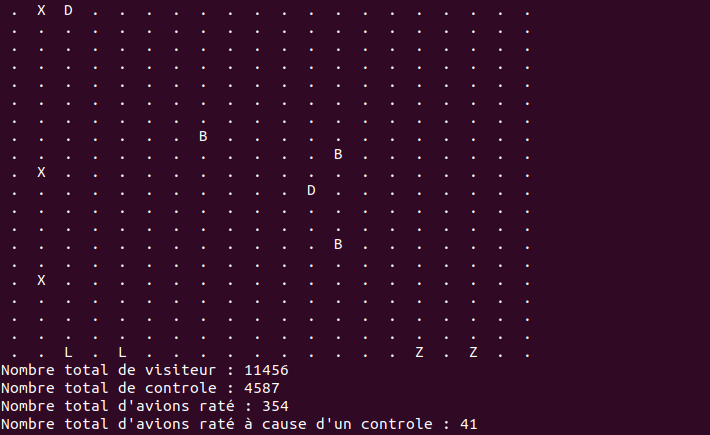
\includegraphics[scale=0.6]{ite.png}
	\caption{Affichage d'une itération type}    
\end{figure}

Nous voyons ci-dessus l'affichage d'une itération type de notre simulation. Pour obtenir des résultats cohérents, nous faisons 100 itérations de cette simulation et calculons alors la moyenne.  
\newline


A la fin de nos itérations, nous voyons qu'en moyenne, 321 personnes ratent leur avions sur 11632 dont 43 à cause d'un des 4613 contrôles de la journée ce qui correspond à 0.02 et 0.003 pour-cent.
Si nous faisions cette simulation pour le compte d'un aéroport, nous pourrions conclure que les douaniers sont responsables d'un nombre assez important de manque d'avions dans un journée type avec ces paramètres.  

\section{Changement de Conception}

Malgré une analyse et une conception poussée en aval de notre SMA, nous avons tout de même légèrement modifié nos diagrammes prévisionnels que nous allons vous présenter ci-dessous.
\newline

La première modification concerne le diagramme de gantt de notre projet.

\begin{figure}[H]
	\centering
	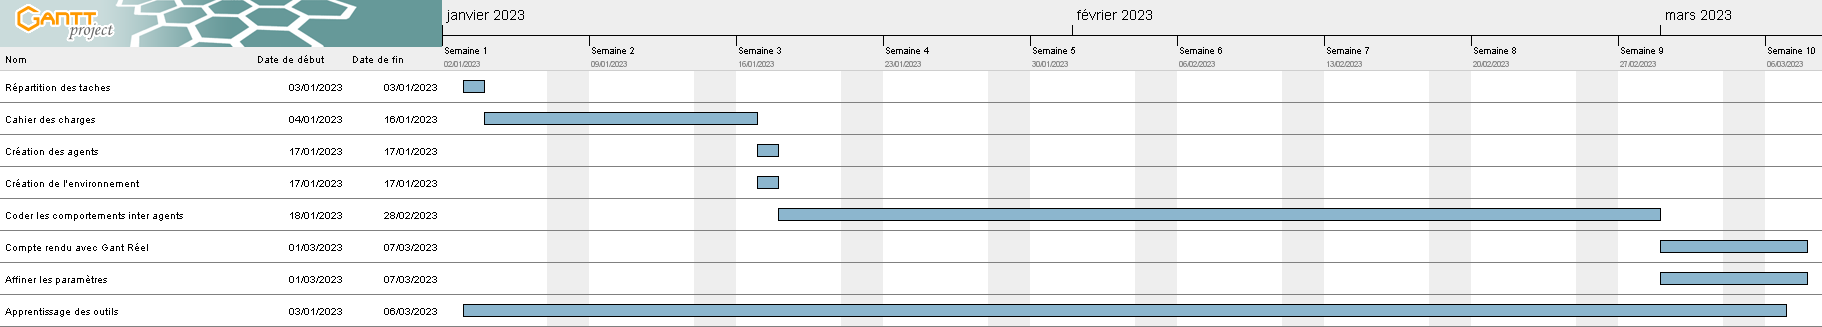
\includegraphics[scale=0.35]{gantt.png}
	\caption{Diagramme de Gantt prévisionnel}    
\end{figure}

\begin{figure}[H]
	\centering
	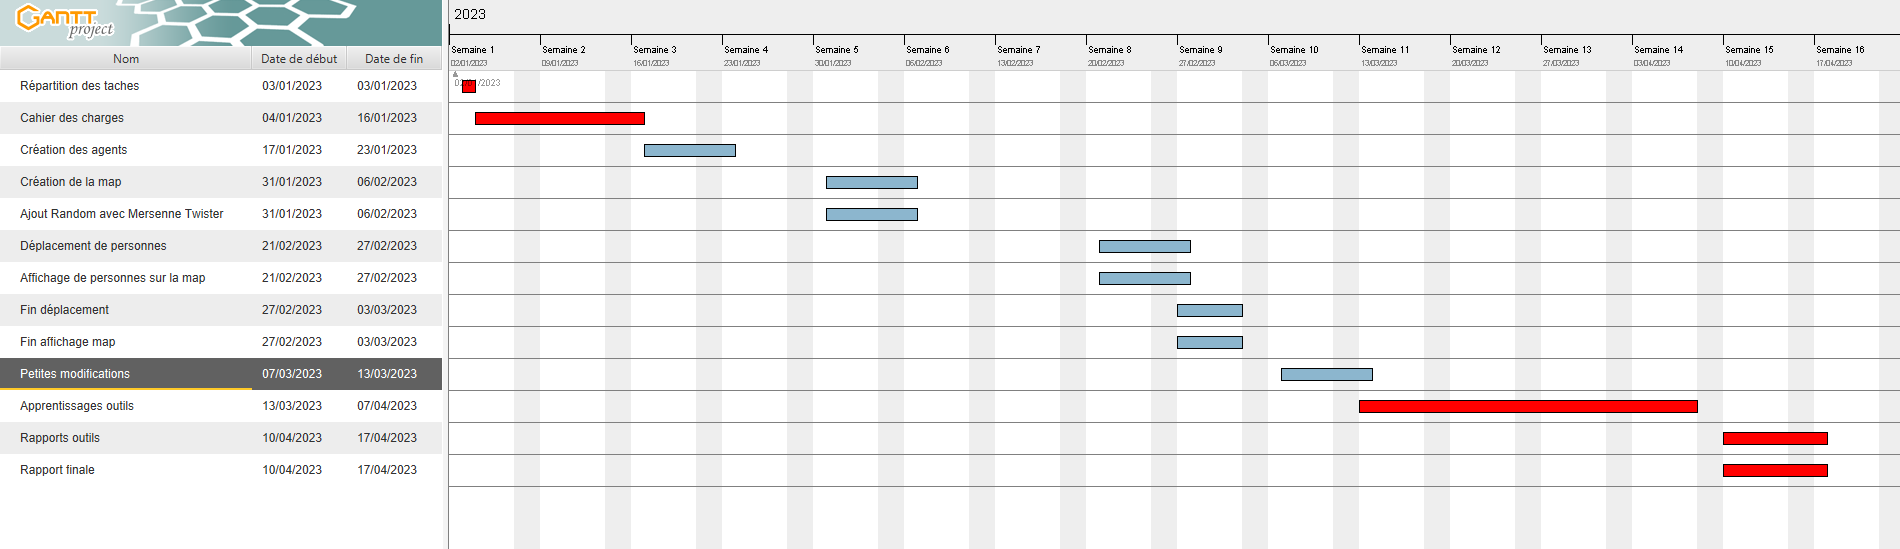
\includegraphics[scale=0.285]{ganntreel.png}
	\caption{Diagramme de Gantt réel}   
\end{figure}
 
 Comme nous pouvons le voir en comparant les deux diagrammes ci-dessous, nous avions un peu sous-estimé le temps que nous possédions pour pouvoir développer ce projet. Pour résoudre ce problème, nous avons étendu les taches de notre projet jusqu'à la date limite. Nous avons aussi séparer la plupart de nos taches pour pouvoir gagner du temps en se les répartissant de manière optimisée. Enfin, nous avons concentré notre temps à la gestion de nos outils à étudier après avoir fini le code de notre simulation multi-agent.
 
 
 Pour ce qui est du diagramme de classe et d'utilisation de notre conception, ils se sont révélés être plutôt précis par rapport à notre conception final. La seul différence étant la gestion de l'aéroport qui a évolué d'une classe à un objet carte disponible pour l'ensemble des objets.

\section{Conclusion}

Pour conclure sur ce projet de simulation multi-agent, nous avons eu la possibilité de travailler et améliorer de nombreuses compétences tout au long de notre projet. La partie analyse et conception nous a permis de travailler et de mettre au gout du jour notre vision de la représentation UML par la création de diagramme de Gantt, de classe mais aussi de cas d'utilisation. Ainsi nous avons pu nous donner quelques indications représentant un cahier des charges sur un projet ou nous étions le concepteur et le client. Ensuite, lors de l'implémentation, nous avons eu la chance de travailler en c++ ce qui nous a donné un temps d'avance sur les révisions de la matière qui était présente au second semestre. Enfin, nous avons tous eu la chance de pouvoir découvrir et  d'approfondir un outil d'aide à la conception de tels programmes.   

\listoffigures


\end{document}
